\documentclass[12pt, titlepage]{article}

\usepackage{amsmath}
\usepackage[margin = 1in]{geometry}
\usepackage{graphicx}
\usepackage{booktabs}
\usepackage{natbib}
\usepackage{array}
\usepackage{caption}
\usepackage{setspace}
\usepackage[colorlinks=true, citecolor=blue]{hyperref}


\title{Association between Breast Cancer and Hepatitis C Virus with Age Controlling}
\author{Amy Traianou\\
  Department of Statistics\\
  University of Connecticut
}

\doublespacing
\begin{document}
\maketitle


\begin{abstract}
In Egypt, Hepatitus C virus infection is a common problem that often impedes treatment
of breast cancer in female patients. While previous work has analyze an associaiton 
between HCV seropositivity and breast cancer diagnosis, this paper will focus on the 
potential confounding of age on the association. We will use Fisher's Exact Test to
estimate the crude estimate of the association and the Mantel-Haenszel method to 
stratify the data between ages. The possible effect of age in the association can
lead to improved care for patients. 


\bigskip
\noindent{\sc Keywords}:
Breslow-Day;
Fisher's Exact Test;
Mantel-Haenszel.
\end{abstract}


\section{Introduction}
\label{sec:intro}

Breast cancer is the world's most prevalent cancer and occurs in 
every country in women at any age after puberty. Therefore,
it's extremely important to determine certain risk factors 
that can help detect breast cancer early and save lives. Research 
is constantly being performed to identify risk factors from lifestyle
factors to genetics \citep{sun2017risk}. Family history is shown to 
be a strong predictor for women developing breast cancer. 

However, recent research is looking into how certain diseases can be a risk 
factor for breast cancer or increase the agression of the cancer. 
Research by the Department of Endocrine and Breast Surgery in China 
focused on Hepatitis B and it's association with breast cancer and found 
HBV is potentially affecting estrogen levels, potentially leading 
to a new way of screening for women \citep{vishnu2016does}. Additionally,
some work has been done with Hepatitis C seropositivity in France, but 
the control group was women with other liver diseases \citep{Larrey2010is}.
Thus, the results can only compare women with certain liver diseases, such as 
hepatitis B, alcoholic liver disease, and hemochromatosis to 
women with Hepatitis C. 

Egypt in particular has the highest prevalence of Hepatitis C, and breast 
cancer is the most common cancer. Thus, an association between the two 
would be extremely benficial. So, this paper will examine if there is an 
association between testing positive for hepatitis C virus and breast cancer 
diagnosis while controlling for age in Egyptian populations. Age is a knwon 
and accepted risk factor of breast cancer; older women are more likely to 
develop tumors \citep{sun2017risk}. Therefore, controlling for age is necessary. 

Inconsistency of Hepatitis C prevalence in different regions of Egypt makes 
it difficult to generalize research to the entire country. This paper will 
focus on a small region within the country with high 
prevalence \citep{Hussein2021high} and make conclusions relevent to a specific 
subgroup. 

Recently on October 6th of 2022, Egyptian Minister of Health Abdel-Ghaffar and 
Qatari Minister of Health Hanan Al-Kuwari met in Doha and agreed to use each 
other's expertise in the health field. The health ministers specifically mentioned research 
in Hepatitis C and breast cancer as an area of interest \citep{arham2022egypt}. 
This meeting emphasizes the importance of diving into Hepatitus C Virus 
and it's association with breast cancer. The Egyptian government has defined 
breast cancer as an area of concern and desires to conduct research within their 
population, which is very minimal at the moment. 

The rest of the paper is organized into several sections. Section~\ref{sec:data}
describes the study done in 2020 to test if HCV seropositivity is associated with 
breast cancer diagnosis in Egyptian population. Section~\ref{sec:methods} 
describes the following statistical methods; Fisher's Exact Test, Breslow-Day test,
and Mantel-Haenszel method. Section~\ref{sec:app} applies the methods to data 
from the study, including stratafied between ages. Section~\ref{sec:discuss} 
concludes the paper.



\section{Data}
\label{sec:data}

The data used in this paper is from a 2020 retrospective case-control 
study based on Egyptian female populations \citep{hussein2020association},
sponsered by Mansoura University in Egypt. The study was conducted with
several goals. The main goals we are interested in are 1. to test if seropositivity
is associated with breat cancer diagnosis in Egyptian population and 
2. to test if HCV-positive patients harbour more agressive breast tumors 
than HCV-seronegative patients. 

The study group consists of 405 patients treated at the Oncology Center 
- Mansoura University in the past 10 years. The data was retrieved from
the hosipital filing system. In order to be included, the patients'
invasive breast cancer must be biopsy-proven. Patients with unknown 
viral marker status, multiple cancer diagnoses and virus-unrelated 
hepatic pathology were all excluded. Additionally, the study measured
two outcome measures. The primary measure was the prevalence of 
HCV seropisitivity, which is defined as being Seropositive for the duration
of the study, an average of 6 months. The secondary outcome measure was
the number of disease related events related to breast cancer diagnosis. 
Disease-free survival was calculated from the time of diagnosis to the
last date of follow up for the study. 

The control group consists of 
data from a previous study, conducted from 2015-2017. There are 145 
females from the same geographic distribution, all with no previous 
cancer diagnosis. The group consists of healthy volunteers or hosipital
patients with no cancer diagnosis. 

In both groups, all patients are above the age of 
18. The ratio of study-to-control was intended to be 1:3.
For this paper, patients are stratified based on age- older patients 
are considered 45 years or above and younger patients are below 45 years. 
The data is summarized in Table~\ref{tab:all}. 


\begin{table}[!h]
  \begin{center}
  \captionof{table}{2x2 Contingency Table for all patients}
\label{tab:all}
\begin{tabular}{rrrr}
  \toprule
  & Breast Cancer & No Cancer Diagnosis & Total\\ 
  \midrule
  HCV Seropositive & 88 & 15 & 103 \\ 
  HCV Seronegative & 317 & 130 & 447 \\ 
  \midrule
  Total & 405 & 145 & 550 \\ 
  \bottomrule
\end{tabular}
\end{center}
\end{table}
 

\begin{table}[!h]
  \begin{doublespace}
    Of the 550 women who were involved in the study, 220 were below 
the age of 45 and 330 were of age 45 or above. Table~\ref{tab:younger} 
and Table~\ref{tab:older} show the break down of seropositivity and 
seronegativity for the stratified age groups.
  \end{doublespace}
  \begin{center}
  \captionof{table}{2x2 Contingency Table for pateints younger than 45}
\label{tab:younger}
\begin{tabular}{rrrr}
  \toprule
  & Breast Cancer & No Cancer Diagnosos & Total\\
  \midrule
  HCV Seropositive & 17 & 2 & 19 \\ 
  HCV Seronegative & 110 & 91 & 201 \\ 
  \midrule
  Total & 127 & 93 & 220 \\ 
  \bottomrule
\end{tabular}
\end{center}
\end{table}

\begin{table}[!htb]
\begin{center}
  \captionof{table}{2x2 Contingency Table for pateints 45 and older}
\label{tab:older}
\begin{tabular}{rrrr}
  \toprule
  & Breast Cancer & No Cancer Diagnosos & Total\\
  \midrule
  HCV Seropositive & 71 & 13 & 84 \\ 
  HCV Seronegative & 207 & 39 & 246 \\
  \midrule 
  Total & 278 & 52 & 330 \\ 
  \bottomrule
\end{tabular}
\end{center}
\end{table}

\vspace{1cm}



\section{Methods}
\label{sec:methods}

To test the association of breast cancer and Hepatitis C seropositivity, one can use
the chi-square or Fisher's Exact test, depending on the
conditions from the sample size \citep{warner2013testing}. Fisher's
exact test is useful for when the normality assumption is violated 
and the expected values of the 2x2 table are too small. The test uses 
the hypergeometric distribution to test if the probabilities are
the same between the two groups. Thus, we can determine if there is 
more of a risk of breast cancer for those with seropositive Hep C.
In the data section, the data was summarized into 2x2 contingency tables.
The generalzied table is shown in Figure~\ref{fig:table}.
The first step is calculate the probability of the original table occuring,
using the hypergeometric pdf:
\begin{equation}
P_a=[\frac{(a+b+c+d)a!b!c!d!}{(a+c)!(b+d)!(a+b)!(c+d)!}]^-1
\end{equation}

Based on the alternative hypothesis, you then calculate the probability of 
all more extreme tables based on the a value. In this paper, p1 is the
probability of having breast cancer given that the patient is seropositive
and p2 is the probability of having breat cancer given that the patient
is seronegative. Then, we want to determine if there is an association,
specifically if the risk of having breast cancer is higher for those who
are seropositive. The alternative hypothesis is that p1 is greater than p2-
which will be tested in the application section.

\begin{figure}[tbp]
  \centering
  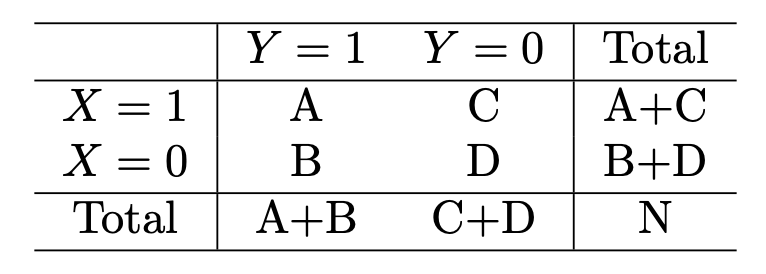
\includegraphics[width=8cm]{table.png}
  \caption{2x2 Contingency Table}
  \label{fig:table}
\end{figure}

\begin{figure}[tbp]
  \centering
  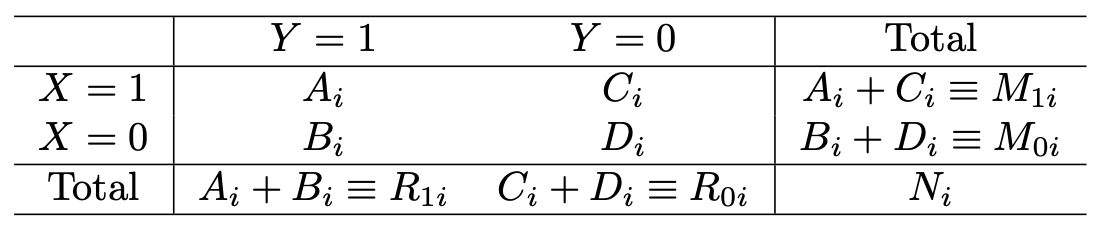
\includegraphics[width=12cm]{2x2 stratified table.png}
  \caption{2x2 Contingency Table with Stratified Data}
  \label{fig:strat}
\end{figure}



After calculating the crude estimate, a Breslow-Day test will test for 
homogeneity of odds ratios between the age stratified data. The generalized
form of stratified 2x2 contingency tables is shown in Figure~\ref{fig:strat}.
The Breslow-Day test statistic will be computed using SAS with the formula:
\begin{equation}
  \chi_{BD}^2=\displaystyle\sum\limits_{i=0}^s\frac{[A_i-E(A_i|\hat{OR}_{M-H})]^2}{Var(A_i|\hat{OR}_{M-H})}
\end{equation}

Based on the results of the Breslow Day test for homogeneity of odds ratios,
the Mantel-Haenszel test will compute a common odds ratio and test if there 
is an association between seropositivity and breast cancer while controlling 
for age. The Mantel-Haenszel test statistic is:
\begin{equation}
  \chi_{M-H}^2=\frac{(|\sum\limits_{i=0}^s A_i - \sum\limits_{i=0}^sE(A_i)|-0.5)^2}
{\sum\limits_{i=0}^s V(A_i)}
\end{equation}

\vspace{1cm}

The expected value and variance of A for the ith strata is 
\[
  E(A_{i})=\frac{M_{i1}R_{1i}}{N_{i}} 
\]
\[
  V(A_{i})=\frac{R_{1i}R_{0i}M_{1i}M_{0i}}{N_i^2(N_{i}-1)}. 
\]


\section{Application}
\label{sec:app}
Fisher's exact test for the pooled data of all patients tested 
\[
H_{0}:p_{1}=p_{2}, H_{a}:p_{1}>p_{2}
\]
at a 0.05 level of confidence.

The test resulted in a p-value of 0.0027, which is less than 
alpha = 0.05. Thus, the null hypothesis is rejected and there 
is evidence suggesting patients who are seropositive have a
higher breast cancer rate than those who are seronegative.

Next, the Breslow Day test checks for homogeneity between the 
stratified ages. 
\[
H_{0}:OR_{1}=OR_{2}, H_{a}:OR_{1}\neq{OR_{2}}
\]
at a 0.01 level of confidence. 

The test resulted in a p-value of 0.0133, which is greater than
the alpha value. Thus, we can conclude the strata have similar
odds ratios and proceed with the Mantel-Haenszel procedure. 

The Mantel-Haenszel test produced a common odds ratio of 1.6847 and 
a 95 percent confidence interval of (0.9283, 3.0574). The interval
contains 1 so after controlling for age, the association is not supported.

However, the individual odds ratios for age groups are worth noting. For 
the older group (45 and older) the odds ratio estimate and interval are 
1.0290 and (0.5197, 2.0374). The odds ratio estimate and interval for the 
younger group (less than 45) are 7.0318 and (1.5828, 31.2399). Therefore,
the association between seropositivity and breast cancer is much stronger
for females less than 45 years. 

\section{Discussion}
\label{sec:discuss}
  Based on the analysis, it is evident that for women under the age of 45,
seropositivity and breast cancer are strongly associated. As being HCV 
positive can complicate treatment of cancer, this is critical information.
In Egypt, breast cancer remains the most common form or cancer and high 
levels of hepatitus C continue. This study was retrospective so analysis 
was limited to observing odds ratios and the sample size was quite small.
Thus, future studies should aim to be prospective cohort studies so 
researchers can observe how seropisitivity and breast cancer interact 
over time. 

Additionally, age is just one factor that can affect the associaiton 
between hepatitus C and breast cancer. Future studies should dive 
deeper into more factors such as weight, reproductive history, 
and alcohol consumption. Addiitonally, future studies can explore how 
seropositivity affects tumor size, disease agression, and more. As 
breast cancer is so prevalent in Egypt, further understanding the 
risk factors is becoming even more important. 

\pagebreak

\bibliography{../manuscript/refs}
\bibliographystyle{chicago}

\end{document}